\section{Autonomous Taxi Fleet Model}
\label{sec:avmodel}

Simulating autonomous taxi services in MATSim requires the implementation, but
even more so a concise planning and definition of how the exact behaviour of
those agents should look like. This will be the first part of this section. Then,
when it is known how those agents can be simulated the next question is how they
should be dispatched for the requests of passengers and finally it has to be decided,
where the autonomous taxis are placed on the network at the beginning of the simulation.
These question will be answered in the second and third part of this section.

\subsection{Agent Behaviour}

The behaviour of an autonomous taxi is not a lot different from an ordinary one,
except that there is no need to roam through the city to find new customers. Therefore,
the AV behaviour presented here is mainly inspired by the model in \todo{cite}, where
ordinary taxi services have been simulated.

The behaviour of an autonomous taxi agent can be described in terms of a task life
cycle. When the agent is not in a task, he is in idle mode, basically (for the basic
model) meaning that he will just stay at the current position and wait for further
instructions. The following steps in the life cycle are depicted in \cref{fig:avstates}.

\begin{enumerate}
\item \textbf{Pickup Drive} is the phase where the AV has got a task and is moving
to the requested pick up location. If the AV is already at the right location, this
point can be skipped, otherwise it represents a leg driving from the current position
to the pickup location.
\item \textbf{Waiting} is the phase in which the AV has arrived at the pickup
location, but the passenger is not there yet. This can only happen if passengers
request cars in advance, prior to the time when they actually want to be picked
up. If the passenger is already present at the time of the arrival at the pickup
location, this state can be skipped.
\item \textbf{Pickup} is the state in which the passenger is picked up. It is
modelled as a fixed time, e.g. one minute and started as soon as both the AV
and the passengers are present at the pickup location.
\item \textbf{Dropoff Drive} represents the leg going from the pickup location to
the dropoff point.
\item \textbf{Dropoff} is the point where the passenger leaves the vehicle. Again,
this is modelled as a fixed time interaction.
\item \textbf{Idle} is the final (and initial) state of the AV life cycle. At this
point the AV will just wait until it receives a new task to pick up another passenger.
\end{enumerate}

The states described above fit very well to the distinction of Activities and Legs
in MATSim as well as to the structure of the AgentFSM framework, which has been
developed for this purpose. Resulting from this behavioural model, a couple of
parameters end implementational questions arise, that can be configured accordingly:

\begin{description}
\item[The Idle behaviour] for the basic model just means that the AV will stay at
its last position. Future extensions could make use of parking facilities or do
an intelligent repositioning to improve the overall performance of the service.

\item[Pickup and Dropoff duration] need to be specified. In accordance with
\todo{cite}, $t_{pickup} = 120s$ and $t_{dropoff} = 60s$ have been chosen. The time
used for the pickup action will not be counted as waiting time (which, in turn,
would be penalized through the marginal utility of waiting as described before).
\end{description}

\begin{figure}
    \centering
    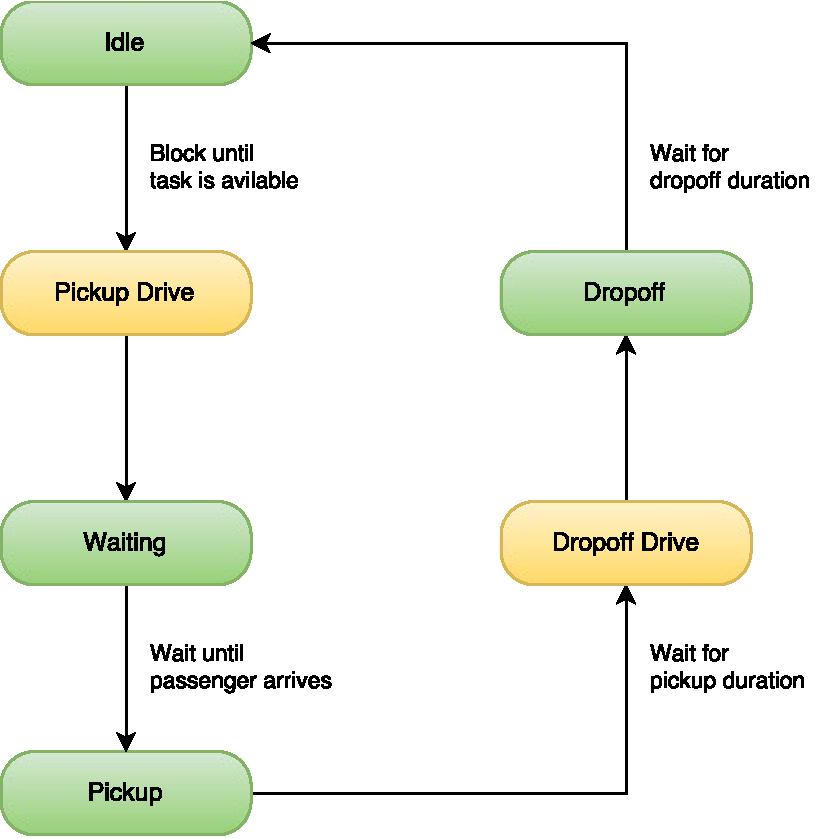
\includegraphics[width=0.7\textwidth]{figures/avstates.pdf}
    \caption{State chart of an AV agent. Activity states are displyed in green, while Leg states are yellow.}
    \label{fig:avstates}
\end{figure}

\subsection{Distribution Algorithm}

At the beginning of a day simulation MATSim all the $n$ available AVs must be placed
somewhere in the network. Two simple distribution algorithms have been implemented
for the purpose of testing in this thesis.

The first one is \textbf{Random Distribution}. Here $n$ links are chosen randomly
from all available network links. While this is an easy distribution strategy for testing,
it create a quite unrealistic scenario. Obviously, in a real AV service, vehicles
would be relcoated over night, such that they can serve as many passengers as
possible during the morning peek.

Therefore a more elaborate distribution strategy has been implemented, which should
lead to more realistic results. Basically one can define a density over the network,
such that every link has a certain probability to get an AV assigned. Then, in $n$
steps, the $n$ available AVs are added to a link dependent on the assignment
probability.

This probability density can be based on many factors. The ones that are implemented
for this thesis are:

\begin{description}
\item[Population density] What is measured here is the population density in terms of
how many people are havingtheir ``home'' activity on a certain link.
\item[AV commuter density] Here for each link it is counted how many people will
have chosen the AV mode for their first leg, i.e. the one that is starting from home.
\end{description}

While the prior one is static, the latter on is dynamic in the sense that for every
iteration in the evolutionary learning, the density will change. So while the
population-density based distribution is a fixed constraint, the latter one captures
the factor of availability. For instance, if there are many agents using AVs in a
certain area, the availability is very high, and thus more people might be inclined
to use it. On the other hand, if availability is low in an area, it might lead to
longer waiting times and people are less likely to use AVs.

While it might be interesting to observe different patterns of availability,
for the first testing purposes the population density is better suited, since a
detailed investigation would need to be done if any results from the AV leg density
come from the mode choice of the agents or of feedback behaviour within the algorithm
itself.

\subsection{Dispatcher Algorithm}

The dynamic dispatching of taxi vehicles is quite a complex scheduling problem,
which is quite hard to solve or needs numerous asumptions to be feasible. In
general, the problem will be a NP hard and heuristical solution strategies need
to be applied if fast solutions are needed. An overview, as well as a proposed
heuristic algorithm can be found in \citet{Maciejewski2015, Bischoff2016}.

The algorithm can be described in two different states:

\begin{description}
\item[Oversupply] occurs when there are more available autonomous vehicles than
requests. This means that each request can be assigned without delay. In that case,
as soon as a request arrives at the dispatcher, the closest vehicle to this request
is searched and assigned to serve the customer.
\item[Undersupply] is the case when all autonomous vehicles are occupied. In that
case requests will stack up, which cannot be handled immediately. In this case the
algorithm works the other way round: As soon as an autonomous vehicle gets available,
it is dispatched to the closest request.
\end{description}

According to the beforementioned papers this strategy gives a near-optimal solution,
although providing fast computational times.

The implementation for this thesis is based on a spatial relaxation of the traffic
network. This means that a grid with a specific resolution in x and y is fitted
over the links. One of these grids saves the locations of all the available AVs,
while another grid saves the locations of all open requests. Because the grids have
a fixed structure, finding the closest AV or request is quite simple, since each
position in x and y belongs to one specific cell of the grid. If no option is found
in a certain cell, the search continues with all cells in its Moore neighborhood
(all 8 surrounding cells). If this still gives no result, the radius is increased
and so forth. When specifiying ``find at least $K$ hits'' as a stop criterion for
a search this resembles an approximate K-nearest-neighbor search based on a $L_1$
norm due to the grid character.
The procedure is depictred in \cref{fig:gridsearch}.

\begin{figure}
    \centering
    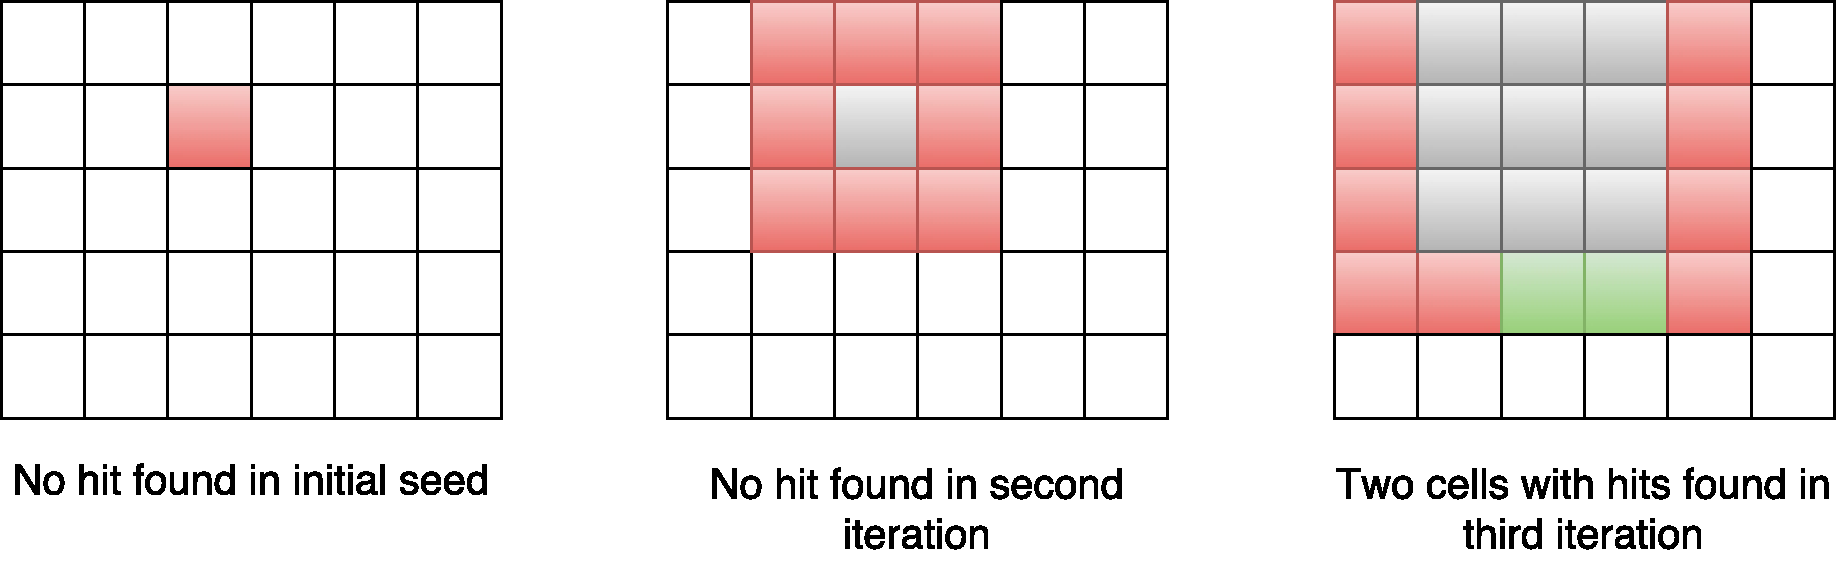
\includegraphics[width=1.0\textwidth]{figures/gridsearch.pdf}
    \caption{Schematic grid search algorithm for the dispatcher}
    \label{fig:gridsearch}
\end{figure}

This search algorithm imposes new parameters to the implementation, which basically
are the cell counts in horizontal and vertical direction. Depending on the topology
of the network, different parameters might be more efficient. If the grid is chosen
to be too dense, many iterations are needed in the algorithm, while a too sparse one
in the extreme case can lead to finding most of the items in only single cell.

In fact, for some topologies it might probably be more efficient to use different
data structures like a binary tree or quadtree to improve the search procedure.
Also more elaborate network search algorithms could be used, which make direct use
of the topology. \todo{cite example maybe}

\todo{Explain how this has been parallelized! Show spoeed improvement!}

For the Sioux Falls scenario it has been tested which impact the choice of the grid
size has on the results. I \cref{fig:gridsize} one can see that very high resolution
grids ($n=200$) lead to a great increase in computational time, due to the necessary
``expansion'' of unoccupied cells, as described above. On the contrary, very low
grid sizes lead to very poor results in terms of the overal average travel time of
the agents, because just selecting a random agent from one of a few cells is basically
just random assignment. A good value for the Sioux Falls network has been found to
be $n=20$, which is computed fastest over the whole range of shares and furthermore
does a good job in decreasing the overall travel time.

\begin{figure}
    \centering
    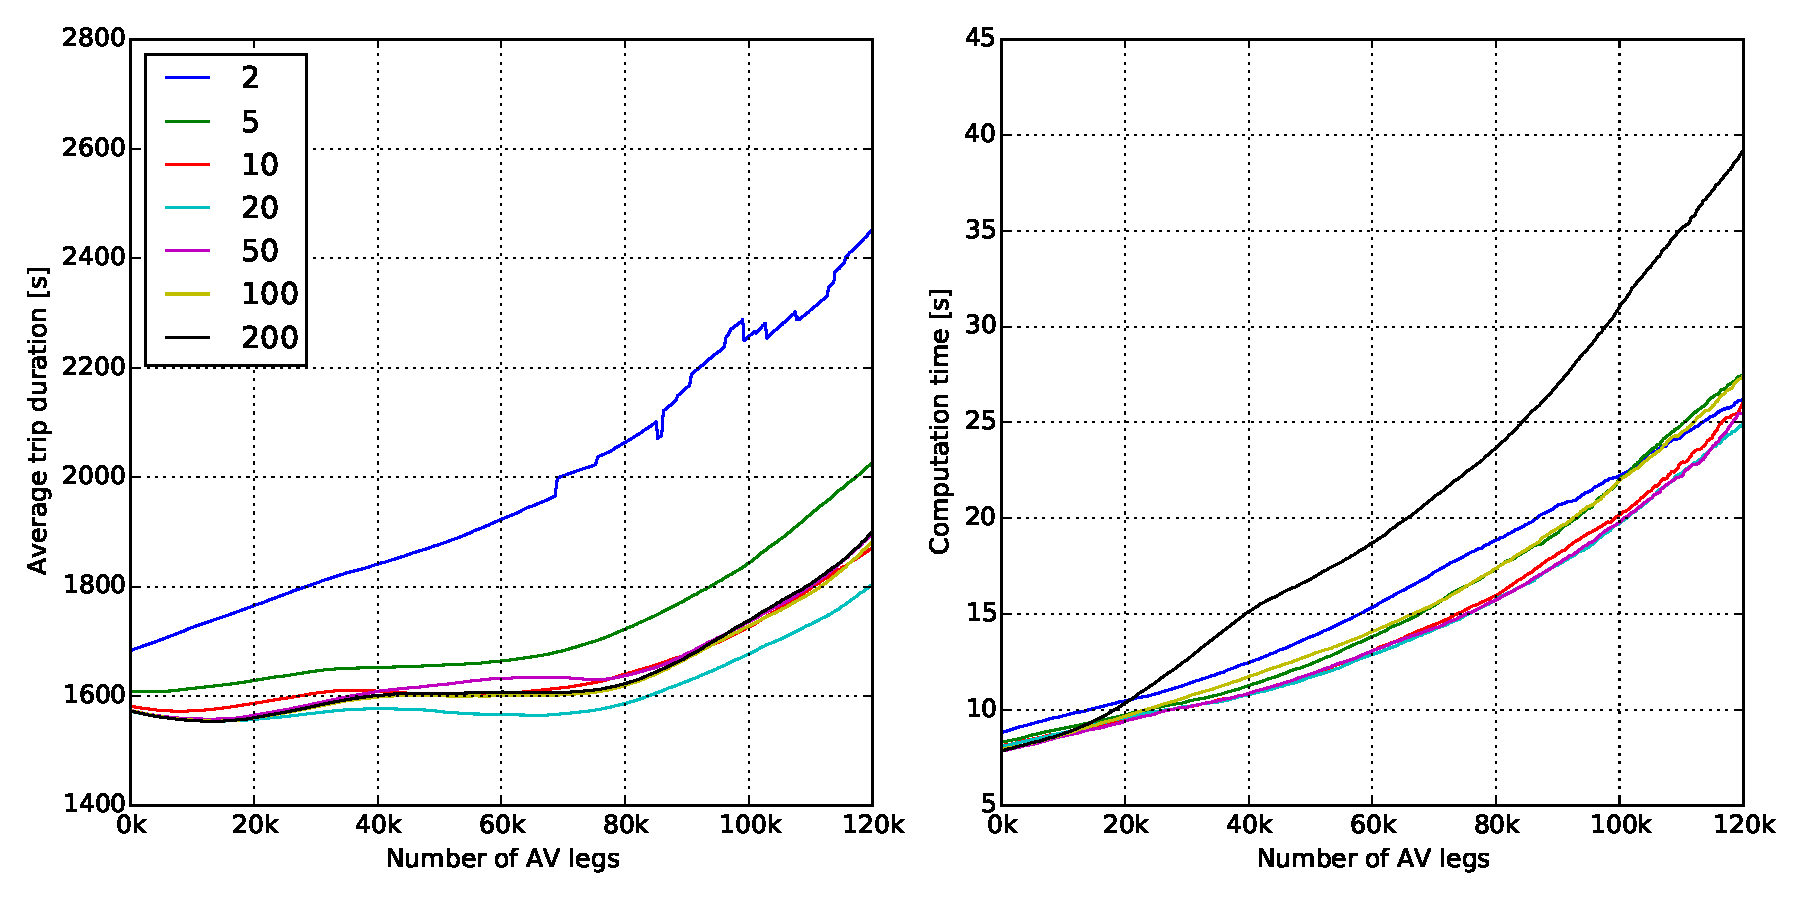
\includegraphics[width=1.0\textwidth]{figures/gridsize.pdf}
    \caption{Performance of different grid sizes in the dispatching algorithm for Sioux Falls}
    \label{fig:gridsize}
\end{figure}

Further improving the dispatching process, the routing has been parallelized. When
the dispatcher is called one per iteration, all the assignments between autonomous
taxi agents and passengers are cached to be processed while the network simulation
of the next iteration is running. Only then, so after one iteration, the dispatcher
waits for all running routing jobs to finish and notifies the agents. This way all
the expensive routing through the network can be done in parallel to the Netsim.
\Cref{fig:routers} shows the impact of adding this feature: While only applying
one parallel router there is already a huge increase in computational performance
compared to the serial processing of the routing tasks. As soon as more routers
work concurrently, this performance is even improved. However, as usual there is
the point where managing the parallelization adds more overhead to the simulation.
For the given scenario a number of routers of $2$ seems to be a reasonable choice.

The parallelization of the dispatcher could be pushed even further. Next to the
routing the actual assignment is the other expensive component in the algorithm.
However, it would probably be hard to parallelize, because concurrent workers
would need to access the same grid structures. The overhead of managing which
worker has access is likely to very fast add more overhead than improvement to
the simulation. One could, however, put the whole assignment process as a serial
procedure in parallel to the Netsim, as done with the routers. This could be a
promising approach of pushing the performance of the simulation even further.

\begin{figure}
    \centering
    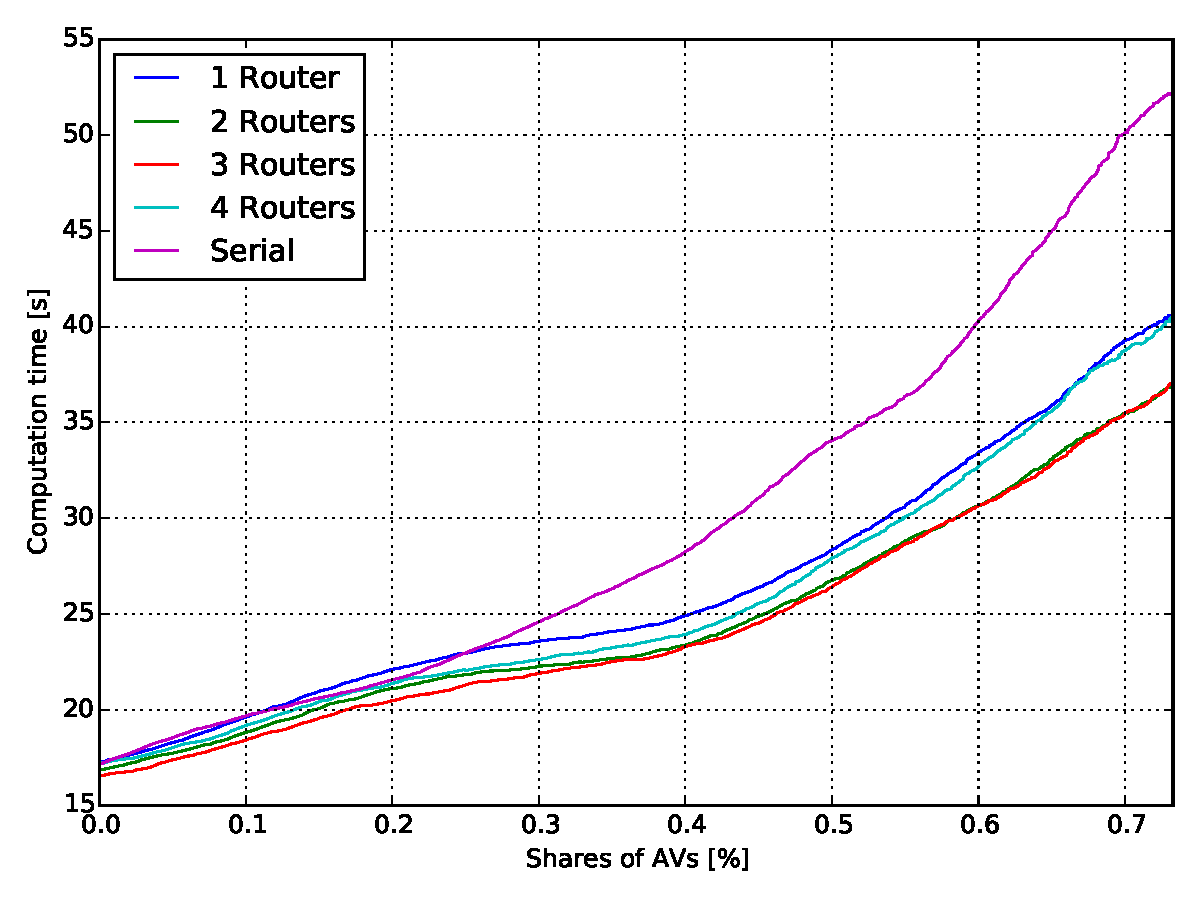
\includegraphics[width=0.7\textwidth]{figures/routers.pdf}
    \caption{\todo{todo}}
    \label{fig:routers}
\end{figure}

\subsection{Routing Algorithm}

The easiest most simple option for routing autonomous vehicles in the model would
be to solve a Dijkstra routing problem through the street network, while minimizing
the expected travel time based on the freespeed values of the links. This strategy
works well for small shares of AVs, because they have not a big impact on the overall
traffic situation.
However, when reaching high shares of AVs one (in simulation as in reality) faces
the problem that the routing cannot be done on the fastest route for most of the
people, as this generates too much congestion. By finding the shortest path in terms
of freespeed, one artificially creates bottlenecks, because all AVs are routed
through the same arterials. This is already an interesting result that can be moved
directly to reality: As soon as an AV operator gains such a high share that he
directly impacts the traffic situation, he must also make sure to relax congestion
in the network, otherwise the service is creating too much of a delay.

In the simulation this got apparent when, for certain shares, huge numbers of
agents could not finish their plans, because all arterials were cluttered by
queueing autonomous taxis. While finding an ``intelligent'' congestion redistribution strategy is a whole
different topic \todo{There are probably interesting publciations, have a look
for that}, for the purpose of simulating AVs in this thesis a rather static approach
is taken. The main idea is to add stochasticity to the Dijkstra process, thus creating
slightly perturbed routes. What needs to be answered for using this approach is,
which magnitude those perturbations should have. In order to solve this problem,
the Sioux-16 baseline scenario has been examined. The 30h day has been divided
into $N=720$ bins ($2min$ each) and for each find the relative decrease in speed for all link
passages starting in each bin has been computed:

\begin{equation}
r_{i,j} = \sum_{j=1}^{n_i} \frac{v_{i,j,freespeed} - v_{i,j,simulated}}{v_{i,j,freespeed}}
\end{equation}

Here $n_i$ is the number of link passages (all agents and all links) that occured
in bin number $i$ and $r_{i,j}$ is the relative decrease of speed in each bin for
each passage.

As can be seen in \cref{fig:speeddecdist}, the distribution of decreases in travel
speeds of the network links can approximated using a Gamma distribution. The outliers,
which can be seen on the right, are those cases where there is a lot congestion in
peak hours. Because those are exactly the cases that one wants to avoid here, they
are ommitted in the following steps.
The assumption of a Gamma-distribution is wholly motivated by the shape of the histogram,
performing an educated derivation of the distribution shape would be an interesting
investigation, which is out of the scope of this thesis though.

A Gamma distribtion is defined by a shape parameter $k$ and a scale parameter $\theta$. For
all bins in the baseline scenario, the respective parameters have been obtained using
the MLE estimator for $\theta$ and a Newton approximation for $k$ as described in
\todo{add citation}. \Cref{fig:randommodel} shows the parameter values for each bin on top,
after they have been smoothed using a moving average filter of length $20$. Also,
for the times before roughly 5am and after 10pm, average parameter values over the
off-peak hours in the middle of the day have been inserted due to a lack of sufficient
data for fitting the speed decreases in these outer areas.

Also shown in \cref{fig:randommodel} (on the bottom) is the mean of the speed decrease at each time of the
day, framed by the $10\%$ and $90\%$ quantiles, now instead of simulation results based on the statistical model.
It can be seen that due to the Gamma model, the range of probable decreases is high in peak hours, up to 70\%,
while the 10\% stays quite constant during the day. The graph of the mean increase suggests that the presented
model is a reasonable approximation, which qualitatively makes sense.

The final travel speed for the router can now be described as a random variable:

\begin{equation}
    V_{i,j,routing} = v_{i,j,freespeed} \cdot (1 + R_i)
\end{equation}

with $R_i \sim \Gamma(k_i, \theta_i)$ being Gamma-distributed for each bin.

The overall effect of this model is then as follows: There is a certain increase
in travel time expected for each link, which depends on its freespeed and the time
of the day. However, especially in peak hours, when the bottlenecks would be a
critical problem, more variation is added to the expected increases in travel time
and thus a better variation in the routing is reached. In each case, the expected
increases are founded on the actual network characteristics of the Sioux-16 network.

What has to be kept in mind is, that this effectively puts a boundary on the
possible number of AVs in the simulation. While the presented approach helps to
avoid too much congestion for a wide range of AV shares, it doesn't perform an
actual intelligent redistribution of congestion in the network. So because of
too much congestion there will be a limit of AVs that can be used, since waiting
times and travel times will get to expensive. This equilibrium generally should
be lower than the actual ``network congestion capacity'' for the theoretical case
of globally optimally routed AVs.

In the same sense it has to be acknowledged that no investigation has been done
to find out how close the proposed model is operating to a theoretical optimum, so
the following results in this thesis have to be understood under the assumption
of this stochastic routing approach and might not represent the best possible
solution.

\begin{figure}
    \centering
    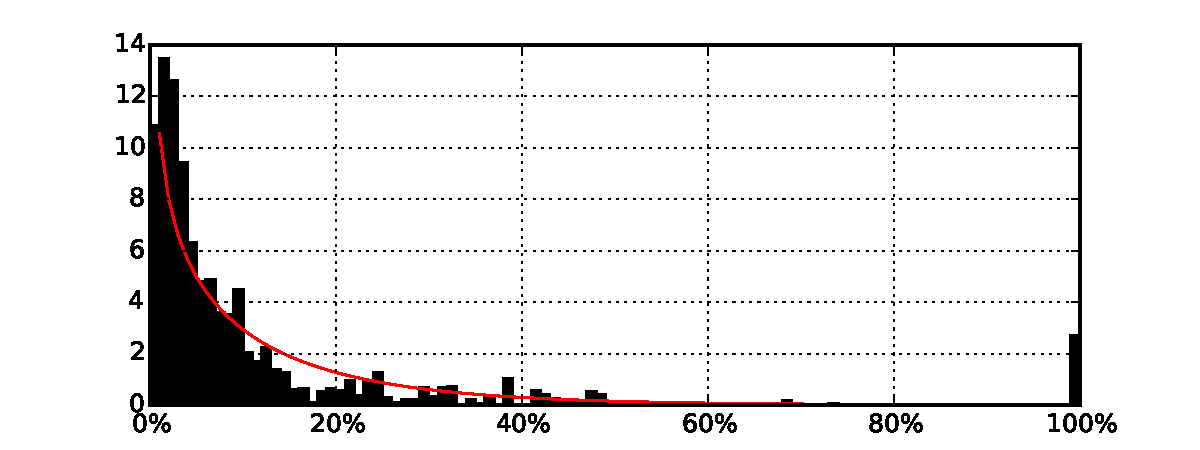
\includegraphics[width=0.5\textwidth]{figures/speeddecdist.pdf}
    \caption{\todo{todo}}
    \label{fig:speeddecdist}
\end{figure}

\begin{figure}
    \centering
    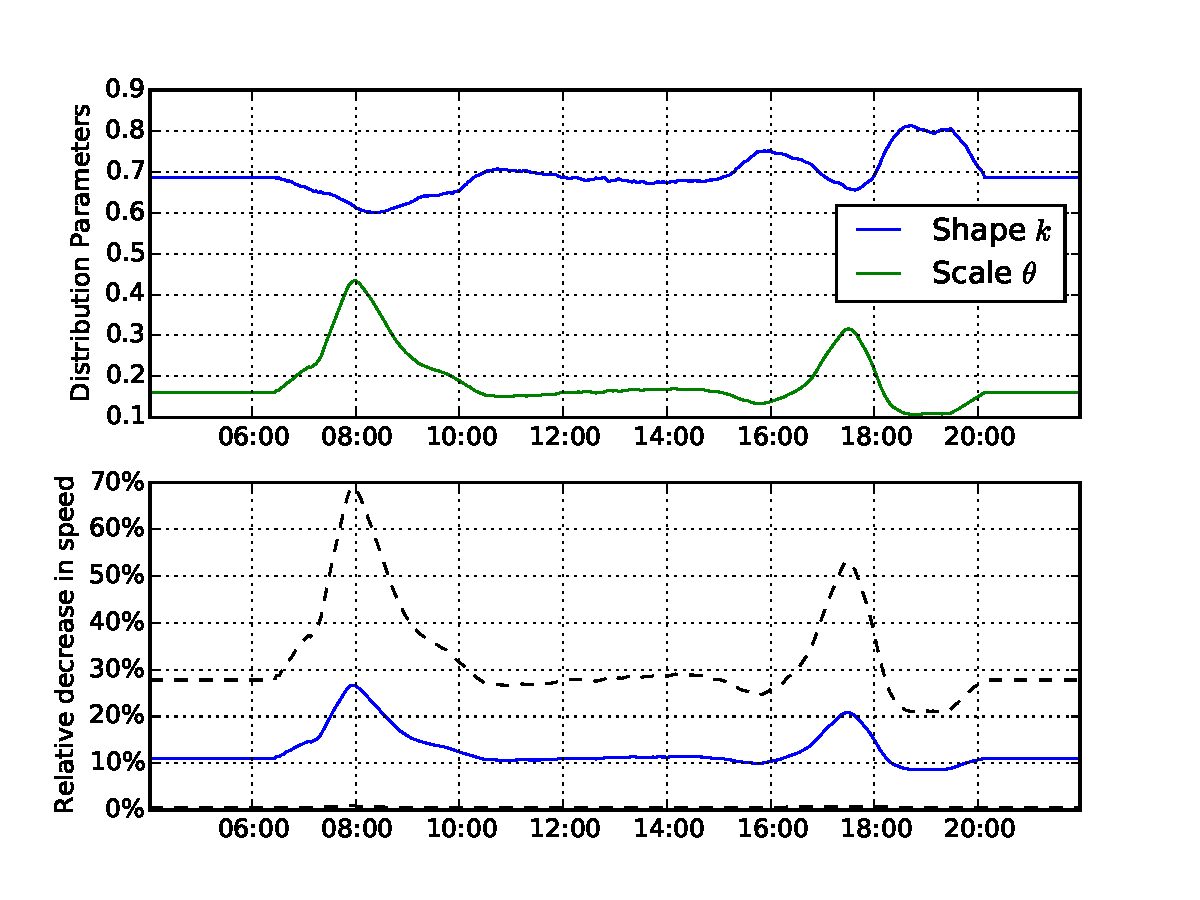
\includegraphics[width=1.0\textwidth]{figures/randommodel.pdf}
    \caption{\todo{todo}}
    \label{fig:randommodel}
\end{figure}
